\chapter{Algoritmus}
\label{kap:algoritmus}
Po preskúmaní triangulačných algoritmov sme sa v našej práci rozhodli venovať čo najkvaitnejšiemu
prevedeniu triangulácie s menším dôrazom na rýchlosť výpočtu. Ako základnú štruktúru sme použili 
postup, ktorí uviedli autori článku \cite{hilton1996marching}. Tento algoritmus využíva 
\textit{Delaunayovu podmienku} predstavenú v kapitole \ref{kap:delaunay_triangulation}.
Daný algoritmus je implementovaný ako prechod cez frontu, v ktorej sa na úvod nachádzajú
hrany počiatočného trojuholníka, v každom kroku vyberieme z fronty jednu hranu $E$ a pre túto
hranu vykonáme nasledujúcu postupnosť krokov:
\begin{enumerate}
    \item{Vytvoríme vrchol $\overrightarrow{x}_{proj}$ tak, ako sme opísali v kapitole \ref{kap:marching_triangles}, teda 
    ako bod ležiaci v kolmej vzdialenosti $k$ od stredu hrany $E = (\overrightarrow{x}_i, \overrightarrow{x}_j)$ 
    v rovine susedného trojuholníka $T$.}
    \item{Nájdeme vrchol $\overrightarrow{x}_{new}$ ako vrchol, ktorý leží na povrchu a je najbližší k bodu 
    $\overrightarrow{x}_{proj}$. 
    Platí teda, že $F(\overrightarrow{x}_{new}) = 0$.}
    \item{Skončíme ak je splnená jedna z nasledujúcich možností:
    \begin{itemize}
        \item{Vrchol $\overrightarrow{x}_{new}$ leží na hranici, teda medzi hraničnými 
        hranami sa nachádza hrana s vrcholom $\overrightarrow{x}_{new}$.}
        \item{Normála $n_{new}$ trojuholníka $T_{new}$ ktorého vrcholy sú $\overrightarrow{x}_i, 
        \overrightarrow{x}_j, \overrightarrow{x}_{new}$ je opačná ako
        normála $\overrightarrow{n}$ susedného trojuholníka $T$, teda 
        $\overrightarrow{n}_{new} \cdot \overrightarrow{n} < 0$.}
    \end{itemize}
    }
    \item{Pre trojuholník $T_{new}$ overíme platnosť \textit{Delaunayovej podmienky}, 
    ktorú sme predstavili v kapitole \ref{kap:delaunay_triangulation}, ak podmienka platí
    vykonáme nasledujúce kroky a prejdeme na ďalšiu hranu.
    \begin{itemize}
        \item{Pridáme vrchol $\overrightarrow{x}_{new}$ medzi hraničné vrcholy.}
        \item{Pridáme trojuholník $T_{new}$ do meshu.}
        \item{Pridáme hrany $(\overrightarrow{x}_i, \overrightarrow{x}_{new})$ a 
        $(\overrightarrow{x}_j, \overrightarrow{x}_{new})$ do fronty s hranami.}
    \end{itemize}
    }
    \item{
        Ak podmienka neplatí overíme platnosť \textit{Delaunayovej podmienky} pre Trojuholníky 
        $T_{prev}$, ktorého vrcholy sú $\overrightarrow{x}_i, \overrightarrow{x}_j, 
        \overrightarrow{x}_{prev}$ a $T_{next}$, ktorého vrcholy sú 
        $\overrightarrow{x}_i, \overrightarrow{x}_j, \overrightarrow{x}_{next}$, kde 
        $\overrightarrow{x}_{prev}$ a $\overrightarrow{x}_{next}$ sú hraničné vrcholy, 
        $\overrightarrow{x}_{prev}$ 
        je sused vrchola $\overrightarrow{x}_i$, $\overrightarrow{x}_{next}$ je sused vrchola 
        $\overrightarrow{x}_j$. Ak niektorý z nich podmienku
        spĺňa, vykonáme preň body z kroku 4 a prejdeme na ďalšiu hranu.
    }
    \item{
        Ak všetky trojuholníky $T_{new}$, $T_{prev}$ ani $T_{next}$ nespĺňajú podmienku, potom 
        ak \textit{Delaunayova guľa} obsajuhe hraničný vrchol $\overrightarrow{x}_{overlap}$ nejakého hraničného 
        trojuholníka $T_{overlap}$, ktorý je rovnako orientovaný ako hraničný trojuholník T, teda
        platí $n*n_{overlap} > 0$, potom overíme platnosť \textit{Delaunayovej podmienky} pre 
        trojuholník $T_{overlap}$ kde $\overrightarrow{x}_{overlap}$ je najbližší k hrane E zo všetkých hraničných
        vrcholov, ktoré sa nachádzajú v Delaunayovej guli. Ak podmienku spĺňa aplikujeme naň body z 
        kroku 4 a prejdeme na ďalšiu hranu.
    }
    \item{
        Ak žiadny trojuholník nebol pridaný do meshu, testovanie hrany E skončíme.
    }
\end{enumerate}

Tento algoritmus používame v našej práci ako základnú štruktúru a pridávame do neho ďalšie podmienky 
a postupy na skvalitnenie výslednej triangulácie. V neadaptívnej verzií volíme vzdialenosť $k$ ako 
výšku rovnostranného trojuholníka so stranou dĺžky zadanej ako vstupný parameter algoritmu, teda 
$\frac{\sqrt{3}}{2}*strana$.

Náš algoritmus je z triedy \textit{Surface Tracking} algoritmov, teda algoritmus sledujúci povrch.
Funguje na princípe postupného pridávania trojuholníkov do rozpracovaného meshu.

Na vstupe algoritmu je implicitne zadaná funkciu $S$, určujúca plochu, ktorú chceme triangulovať. 
Zadaná plocha musí byť hladká, teda bez singularít.
Takisto máme zadanú veľkosť hrany $a$ trojuholníka, toto je priližná veľkosť hrany trojuholíka v 
triangulácii. Čím je veľkosť hrany menšia, tým je triagulácia presnejšia. Veľkosť hrany trojuholníka 
nesmie byť príliš veľká. Malá veľkosť hrany zvyčajne nevadí, avšak pre menšie trojuholníky trvá 
algoritmus omnoho dlhšie. Na vstupe je takisto počiatočný bod v ktorom začneme trianguáciu povrchu.
Tento bod musí ležať na povrchu.
Začneme vytvorením jediného trojuholníka s veľkosťou hrany približle $a$, presný spôsob implementácie
opíšeme v kapitole TODO.

Funkčnosť algoritmu opíšeme akosi indukčne. Majme korektnú čiastočnú trianguáciu povrchu, na začiatku
je to jediný trojuholník. Prvá otázka ktorú si pokladáme je nasledujúca. 
\textit{Aké podmienky musí spĺňať trojica vrcholov} $x_i, x_j, x_{new}$ 
\textit{aby sme ju pridali do triangulácie ako nový trojuholník na hraničnej hrane} $E = (x_i, x_j)?$ 

\section{Pridanie trojuholníka do meshu}
\label{kap:triangle_conditions}

Majme hraničnú hranu $E=(x_i, x_j)$ čiastočnej triangulácie $M$ a bod $x_k \in \mathbb{E}^3$. 
Tento bod sa môže aj nemusí nachádzať medzi vrcholmi $M$. Za akých podmienok môžeme pridať trojuholník 
$T=(x_i, x_j, x_k)$ do $M$?

\begin{itemize}
    \item{
        Trojica bodov tvorí trojuholník.


        Veľmi zjavná avšak veľmi dôležitá podmienka. Prakticky overenie tejto podmienky znamená overenie
        známej \textit{trojuholníkovej nerovnosti}.  
    } 

    \item{
        Trojuholník je správne orientovaný.


        Čo znamená správna orientácia môžeme vidieť na obrázku \ref{obr:good_orientation}. Uhol $\beta$
        počítame ako uhol dvoch vektorov $\overrightarrow{x_i x_j}$ a $\overrightarrow{x_i x_{new}}$, 
        pričom nás zaujíma nie len veľkosť uhla ale aj orientácia vzhľadom na susedný trojuholník, čo 
        vyjadríme znamienkom pri veľkosti uhla. 

        \begin{figure}
            \centerline{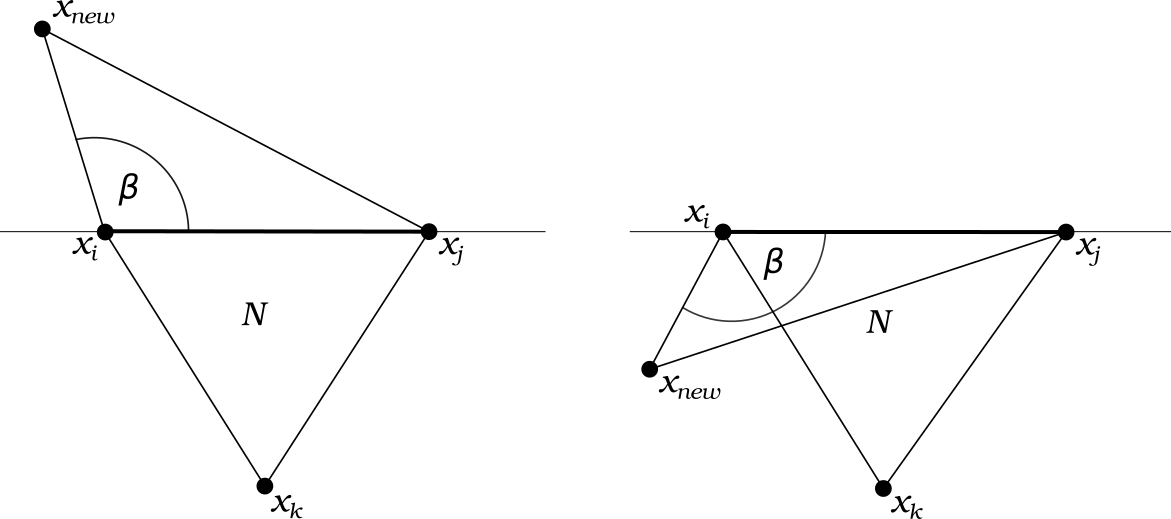
\includegraphics[width=0.55\textwidth]{images/good_orientation}}
            \caption[]{$T(x_i, x_j, x_{new})$ \textit{naľavo} má správnu orientáciu, \textit{napravo} má nesprávnu.}
            %id obrazku, pomocou ktoreho sa budeme na obrazok odvolavat
            \label{obr:good_orientation}
        \end{figure}

        Pod orientáciou vzhľadom na susedný trojuholník myslíme nasledovné.
        Ak

        $$(\overrightarrow{x_i x_j} \times \overrightarrow{x_i x_k}) 
        \cdot (\overrightarrow{x_i x_j} \times \overrightarrow{x_i x_{new}}) < 0$$

        tak je uhol v intervale $(0, \pi)$, inak je uhol v intervale $<-\pi, 0>$.
        
        Intuícia za predchádzajúcim vzťahom je taká, že vektorový súčin 
        $\overrightarrow{x_i x_j} \times \overrightarrow{x_i x_k}$ ukazuje \textit{do obrazovky}.
        Vektorový súčin $\overrightarrow{x_i x_j} \times \overrightarrow{x_i x_{new}}$ ukazuje 
        \textit{von z obrazovky} v prípade naľavo, avšak \textit{do obrazovky} v prípade napravo.
        Skalárny súčin týchto smerov je kladný práve vtedy, keď ukazujú \textit{tým istým smerom}, 
        teda ich uhol je menej ako $\frac{\pi}{2}$. 
        
        Trojuholník má \textit{správnu orientáciu} vzhľadom
        na susedný trojuholník $N$, práve vtedy keď uhol $\beta \in (0, \pi)$. V našej implementácii 
        však nechceme príliš úzke trojuholníky, túto podmienku sme teda upravili na podmienku
        $\beta \in (\frac{\pi}{10}, \frac{9\pi}{10})$. Vizualizáciu oblasti, z ktorej sú vhodné 
        vrcholy pre trojuholník $T$ a jeho hraničnú hranu $E$ môžeme vidieť na obrázku 
        \ref{obr:good_orientation_points}.

        \begin{figure}
            \centerline{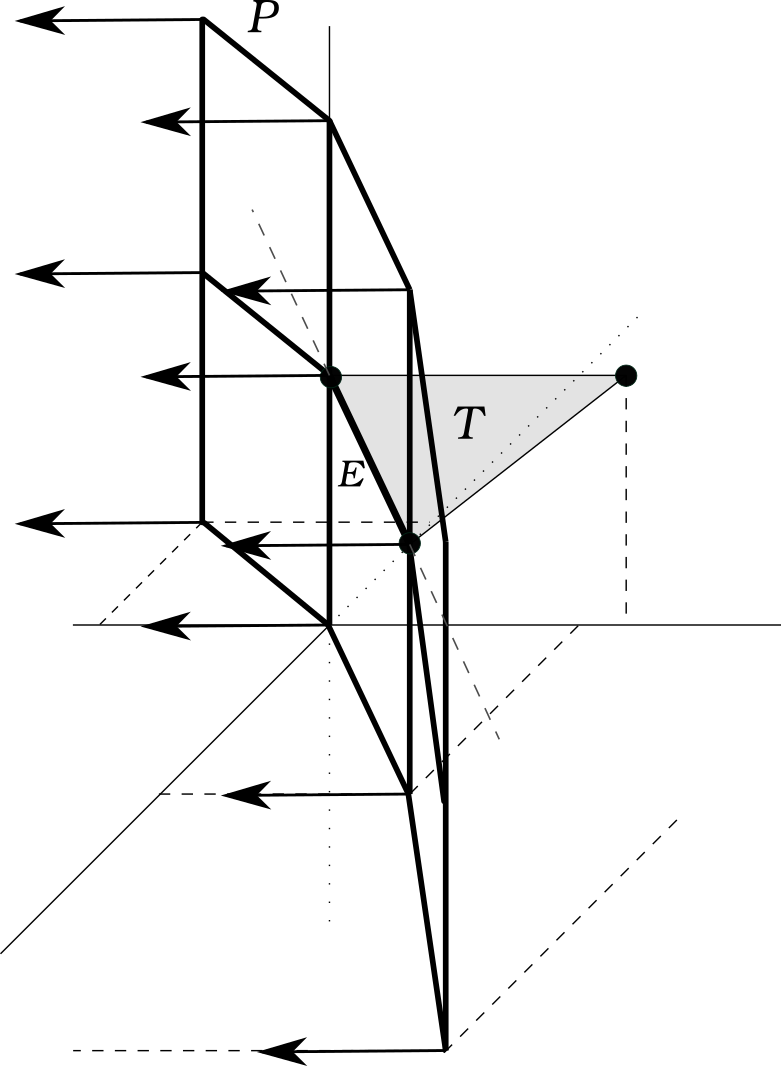
\includegraphics[width=0.25\textwidth]{images/good_orientation_points}}
            \caption[]{Vyhovujúce body sa nachádzajú \textit{naľavo} od plochy $P$.}
            %id obrazku, pomocou ktoreho sa budeme na obrazok odvolavat
            \label{obr:good_orientation_points}
        \end{figure}


        //TODO toto je zle formulované

        Oblasti, v ktorých by sme potrebovali aby mali susedné trojuholníky sklalárny súčin normál menší ako 
        $\frac{\pi}{2}$ sú oblasti s veľkým zakrivením a potrebujeme buď zmenšiť veľkosť hrany trojuholníka
        pre celý model alebo v adaptívnej verzii v takýchto oblastiach prispôsobiť veľkosť trojuholníkov. 
    }

     \item{
         Pre nové hrany $(x_i, x_{new})$ a $(x_j, x_{new})$ platí jedna z nasledujúcich podmienok
         \begin{enumerate}
            \item {
                Hrana je \textit{nová}, teda sa nenachádza medzi doterajšími hranami meshu. 
            }
            \item {
                Ak sa hrana nachádza v meshi, tak je \textit{hraničná}.
            }
         \end{enumerate}
     }

     \item{
         Pre trojuholník je splnená \textit{Delaunayova podmienka} tak, ako bola opísaná v 
         definícii \ref{def:delaunay_constraint}.

        Ako neskôr uvidíme, túto podmienku nemusia nutne spĺňať všetky trojuholníky. Náš algoritmus sa bude 
        skladať z dvoch častí, v prvej časti vyžadujeme od všetkých trojuholníkov splnenie tejto podmienky.
        Po skončení prvej časti zostávajú v meshi diery, ktoré je možné vyplniť trojuholníkmi nespĺňajúcimi 
        \textit{Delaunayovu podmienku}. Príklad takejto diery môžeme vidieť na obrázku 
        \ref{obr:non_delaunay_triangle}. Hrubšie hrany vyjadrujú hraničné hrany triangulácie. 
        Vidíme, že chceme vytvoriť trojuholník $T = (x_i, x_j, x_k)$
        keďže je to jediný spôsob ako uzavrieť dieru v takmer kompletnej triangulácii,
        avšak tento trojuholník nespĺňa \textit{Delaunayovu podmienku}.
     }

     \item{
         V okolí bodu $x_{new}$ sa nenachádza ťažisko už existujúceho trojuholníka.

         Táto podmienka, tak isto ako \textit{Delaunayova podmienka}, nebude musieť byť splnená vždy,
         avšak taktiež ju vyžadujeme v prvej časti algoritmu.
     }
    \begin{figure}
        \centerline{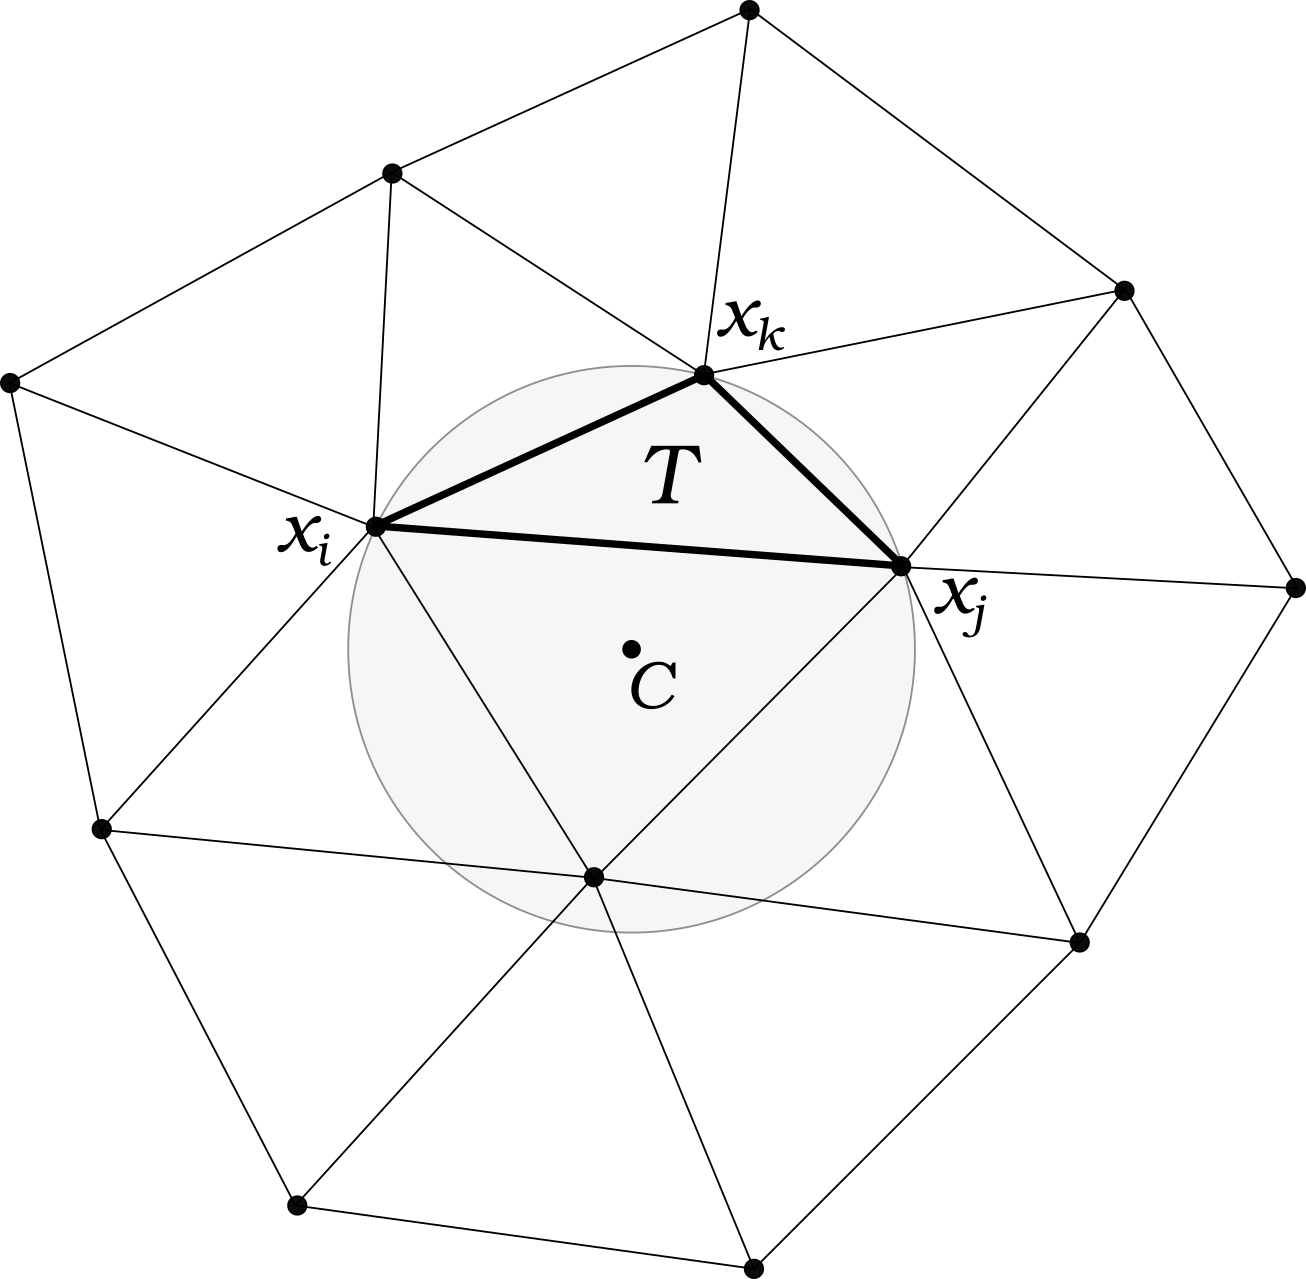
\includegraphics[width=0.35\textwidth]{images/non_delaunay_triangle}}
        \caption[]{TODO}
        %id obrazku, pomocou ktoreho sa budeme na obrazok odvolavat
        \label{obr:non_delaunay_triangle}
    \end{figure}
\end{itemize}

\section{Tvorba nového trojuholníka $T_{new}$}

Majme hraničnú hranu $E=(x_i, x_j)$ čiastočnej triangulácie $M$. V tejto podkapitole opíšeme 
aké vrcholy $x$ skúšame pre túto hranu. Ako sme už spomínali, algoritmus používa ako 
základnú štruktúru postup opísaný na začiatku kapitoly \ref{kap:algoritmus}. 
Do tohto postupu sme však pridali zmeny založené na našich pozorovaniach.

\subsection{Problémy pri tvorbe nového vrchola $x_{new}$}

V tejto podkapitole opíšeme problémy ktoré sme spozorovali počas štúdia základného 
algoritmu.

\begin{enumerate}

\item{
    Ako prvý problém vnímame nespájanie bodov, ktoré sa k sebe nachádzajú blízko. Ako dôsledok vznikajú 
    neskôr úzke alebo malé trojuholníky. Príklad takétoho správania môžeme vidieť na obrázku 
    \ref{obr:first_problem}. Keďže trojuholník $T_{new}$ spĺňa Delaunayovu podmienku, tak podľa 
    základného algoritmu pridáme trojuholník do meshu. Zdalo by sa nám však správne vytvoriť a 
    pridať do meshu trojuholník $\overrightarrow{x}_i, \overrightarrow{x}_j, \overrightarrow{x}_{prev}$. 

    \begin{figure}
        \centerline{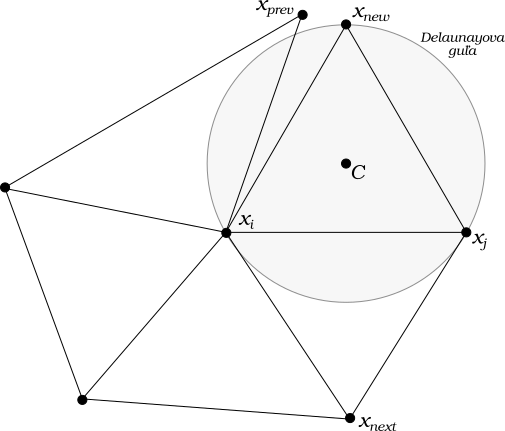
\includegraphics[width=0.35\textwidth]{images/first_problem}}
        \caption[Trojuholník $T_{new}$ spĺňa Delaunayovu podmienku]{Trojuholník $T_{new}$ spĺňa Delaunayovu podmienku}
        %id obrazku, pomocou ktoreho sa budeme na obrazok odvolavat
        \label{obr:first_problem}
    \end{figure}
}

\item{
    Ďalší problém, ktorý vnímame je pretínanie trojuholníkov. Na obrázku \ref{obr:second_problem} môžeme
    vidieť trojuholník $T_{new}$, ktorého nový vrchol $\overrightarrow{x}_{new}$ nemá žaidne blízke body. 
    Pre tento trojuholník je taktiež splnená \textit{Delaunayova podmienka}, teda by sme ho mali pridať 
    do meshu. Vidíme však, že tento trojuholník sa môže pretínať s iným hraničným trojuholníkom.

    \begin{figure}
        \centerline{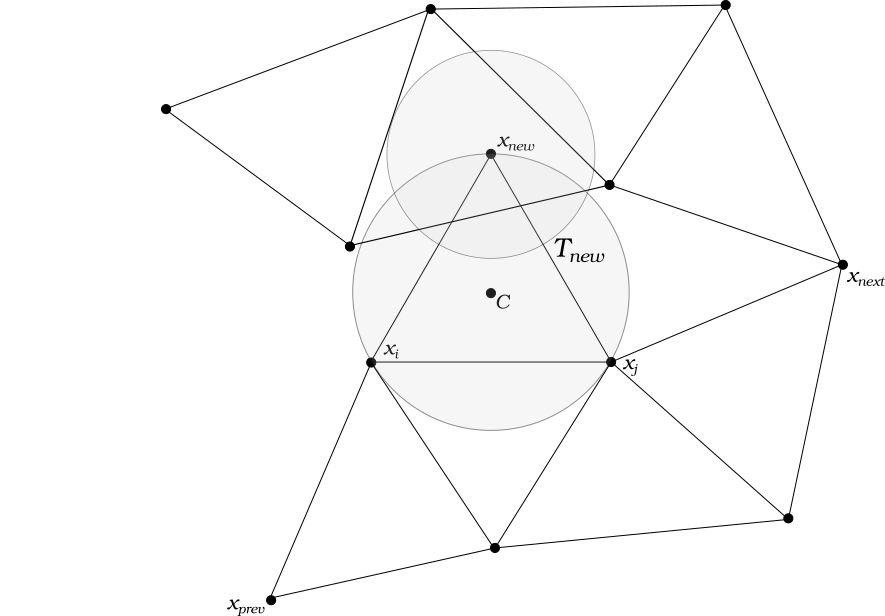
\includegraphics[width=0.5\textwidth]{images/second_problem}}
        \caption[Trojuholník $T_{new}$ nemá vo svojom okolí blízky bod]{Trojuholník $T_{new}$ nemá vo svojom okolí blízky bod}
        %id obrazku, pomocou ktoreho sa budeme na obrazok odvolavat
        \label{obr:second_problem}
    \end{figure}
}

\end{enumerate}
  
\subsection{Navrhované riešenia}

\begin{enumerate}
\item{
    Našim navrhovaným riešením je v okolí vrchola $\overrightarrow{x}_{new}$ pridať guľu s polomerom 
    $0.4-$násobku dĺžky strany trojuholníka. Následne zisťujeme, či sa vnútri tejto gule nachádzajú 
    hraničné body. Tieto body nazveme blízke body k bodu $\overrightarrow{x}_{new}$. V ďalšom kroku 
    sa pokúšame vytvoriť trojuholník s hranou E a blízkymi bodmi počnúc od najbližšieho k hrane $E$. 
    $2D$ ilustáciu riešenia môžeme vidieť na obrázku \ref{obr:first_problem_solution}. 

    \begin{figure}
        \centerline{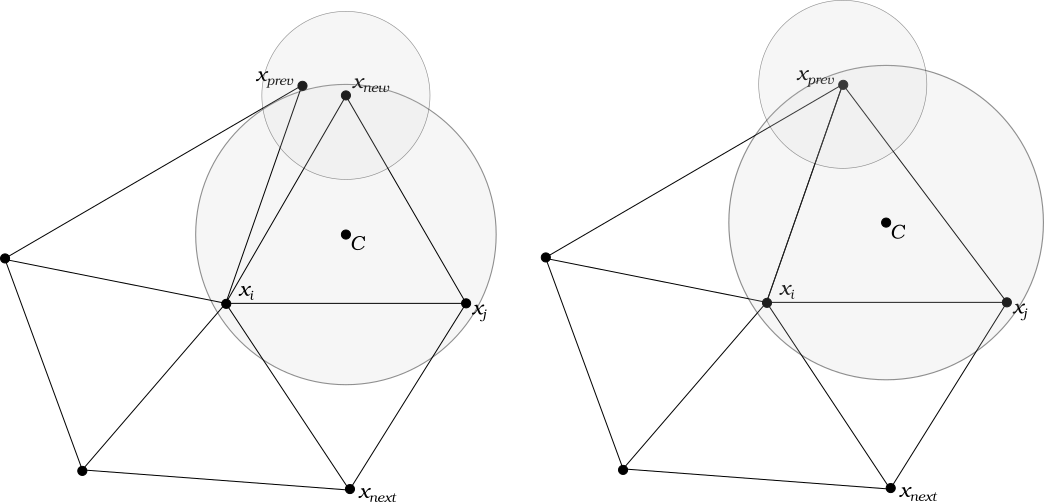
\includegraphics[width=0.7\textwidth]{images/first_problem_solution}}
        \caption[Trojuholník $T_{new}$ má vo svojom okolí blízky bod]{Trojuholník $T_{new}$ má vo svojom okolí blízky bod}
        %id obrazku, pomocou ktoreho sa budeme na obrazok odvolavat
        \label{obr:first_problem_solution}
    \end{figure}
}

\item{

    Naše navrhované riešenie druhého problému je hneď po kontrole blízkych bodov k bodu 
    $\overrightarrow{x}_{new}$ nájsť spomedzi hraničných hrán najbižšiu hranu k bodu $x_{mid}$
    ktorý je stredom hrany $E$. 
    Metrika ktorú používame na nájdenie najbližšej hrany k bodu je definovaná nasledovne.

    \begin{definition} Vzdialenosť hrany $E=(A,B)$ a vrchola $P$ definujeme ako
    \label{def:segment_point_distance}
    \begin{itemize}
        \item{
            $|AP|$ ak $\measuredangle BAP \in (\frac{\pi}{2}, \frac{3\pi}{2})$
        }

        \item{
            $|BP|$ ak $\measuredangle ABP \in (\frac{\pi}{2}, \frac{3\pi}{2})$
        }

        \item{
            $|EP|$ inak
        }

        
        Pričom $|AP|$, $|BP|$ je euklidovská vzdialenosť bodov v $\mathbb{R}^3$ a $|EP|$ je kolmá 
        vzdialenosť bodu $P$ od priamky na ktorej leží hrana $E$.
    \end{itemize}

    \end{definition}

    Vizualizáciu tejto metriky môžeme vidieť na obrázku \ref{obr:edge_vertex_distance}.

    \begin{figure}
        \centerline{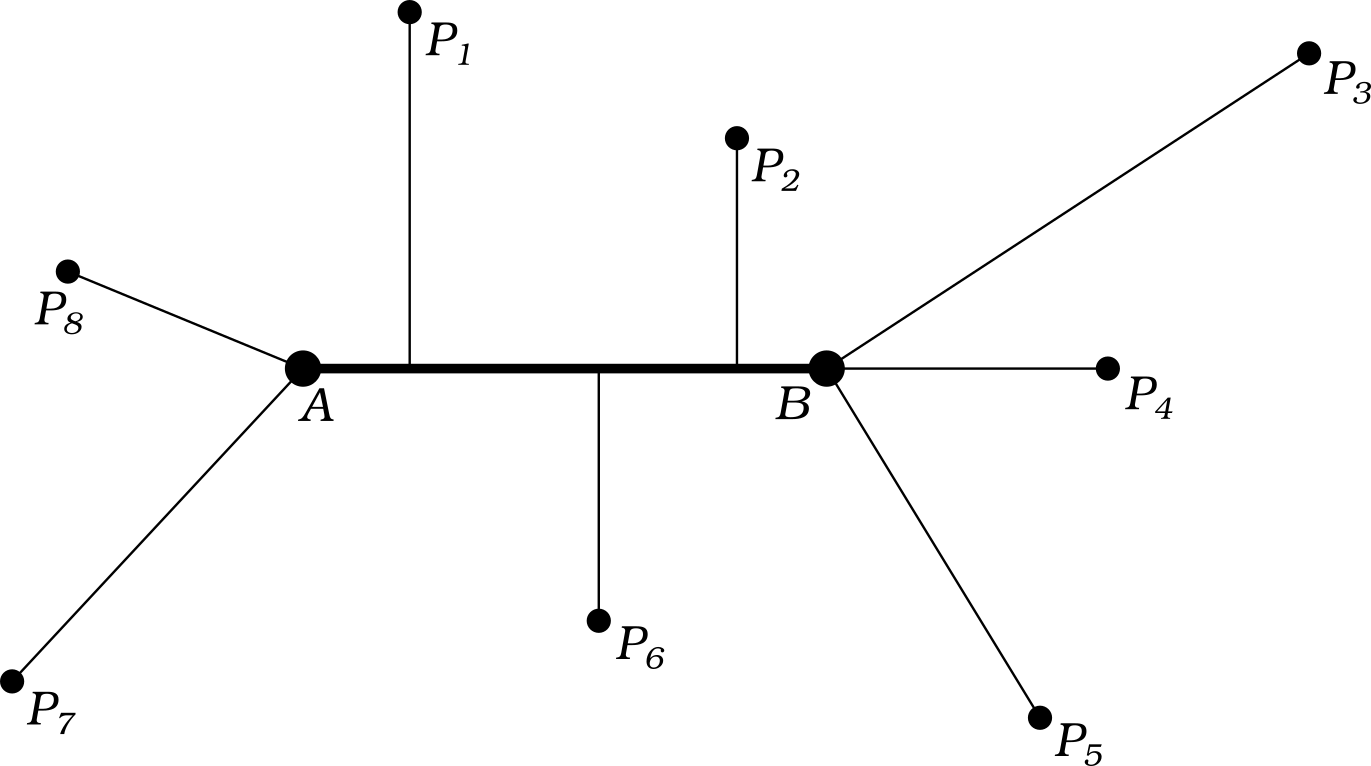
\includegraphics[width=0.6\textwidth]{images/edge_vertex_distance}}
        \caption[Vizualizácia vzdialenosti bodov $P_1, ..., P_8$ od hrany $E=(A,B)$]
        {Vizualizácia vzdialenosti bodov $P_1, ..., P_8$ od hrany $E=(A,B)$}
        %id obrazku, pomocou ktoreho sa budeme na obrazok odvolavat
        \label{obr:edge_vertex_distance}
    \end{figure}

    Po nájdení najbližšej hrany $E_{closest} = (\overrightarrow{x}_k, \overrightarrow{x}_l)$ 
    k bodu sa pokúsime vytvoriť trojuholník z hrany $E$ a vrchola $\overrightarrow{x}_k$, potom z
    vrchola $\overrightarrow{x}_l$. Ak ani jeden z týchto trojuholníkov nie je vhodný, pokúsime sa 
    vytvoriť trojuholník z hrany $E$ a vrchola $\overrightarrow{x}_{mid}$. Tento vrchol 
    volíme ako stred hrany $E_{closest}$, ktorý sprojektujeme na plochu. Ak je tento trojuholník vhodný
    postupujeme nasledovne. 
    
    \begin{itemize}
    \item{
        Vyberieme z meshu trojuholník z ktorého je hrana $E_{closest}$, označme ho 
        $T_{closest}=(x_k, x_l, x_{closest})$.
    }
    \item{
        Rozdelíme trojuholník $T_{closest}$ na dva trojuholníky $T_1 = (x_k, x_{mid}, x_{closest})$ a
        $T_1 = (x_{mid}, x_l, x_{closest})$.
    }
    \item{
        pridáme trojuholníky $T_1$ a $T_2$ do meshu. 
    }
    \end{itemize}

    Tento postup môžeme vidieť na obrázku \ref{obr:second_problem_solution}.

    \begin{figure}
        \centerline{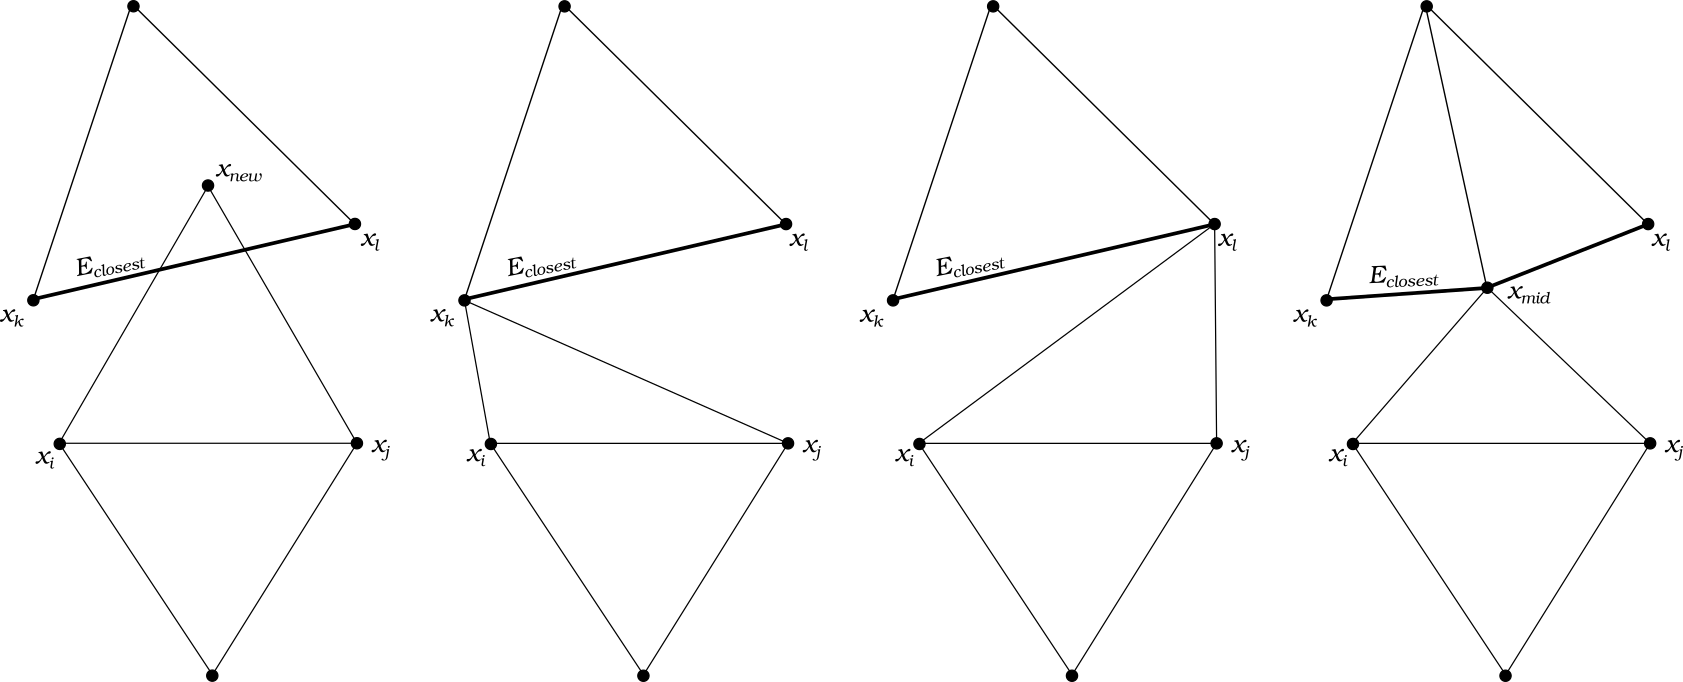
\includegraphics[width=1\textwidth]{images/second_problem_solution}}
        \caption[TODO]{TODO}
        %id obrazku, pomocou ktoreho sa budeme na obrazok odvolavat
        \label{obr:second_problem_solution}
    \end{figure}

    Z toho istého dôvodu sme rozšírili \textit{Delaunayovu podmienku} o podmienku, že 
    v okolí nového vrchola $x_{new}$ sa nesmie nachádzať ťažisko už existujúceho trojuholníka.
    Vizualizáciu tejto podmienky môžeme vidieť na obrázku \ref{obr:centroid_in_delaunay}.

    \begin{figure}
        \centerline{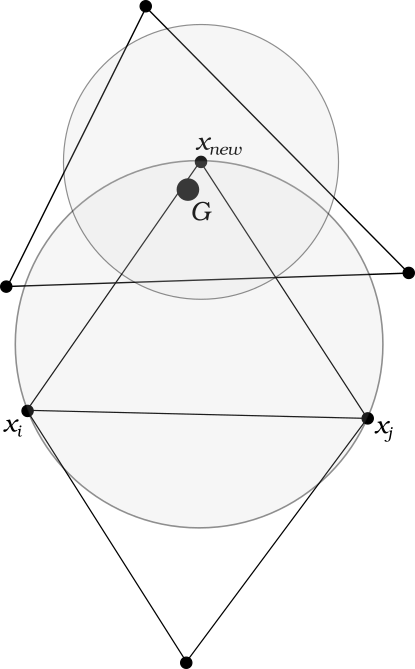
\includegraphics[width=0.25\textwidth]{images/centroid_in_delaunay}}
        \caption[TODO]{TODO}
        %id obrazku, pomocou ktoreho sa budeme na obrazok odvolavat
        \label{obr:centroid_in_delaunay}
    \end{figure}
}
\end{enumerate}

Ak sa nám doteraz nepodarilo vytvoriť žiadny trojuholník s hranou $E$ a zároveň trojuholník 
$T_{new} = (x_i, x_j, x_{new})$ spĺňa všetky podmienky vymenované v podkapitole 
\ref{kap:triangle_conditions}, pridáme ho do meshu. A posunieme sa k ďalšej hraničnej hrane.

\subsection{Skúšanie súsedných hraničných hrán}
Pre zhrnutie uvedieme kroky, z ktorých sa skladal doterajší postup.
\begin{itemize}
\item{
    Vytvorenie nového vrchola $x_{new}$.
}
\item{
    Skúšanie vytvárania trojuholníka s blízkymi bodmi k bodu $x_{new}$.
    Ak sa to podarí, skončíme. 
}
\item{
    Nájdenie najbližšej hraničnej hrany $E_{closest}$.
}
\item{
    Skúšanie vytvárania trojuholníka s koncovými bodmi hraničnej hrany $E_{closest}$ a 
    stredným bodom $x_{mid}$. Ak sa to podarí, skončíme.
}
\item{
    Overenie podmienok opísaných v časti \ref{kap:triangle_conditions}. Ak sú splnené, pridáme do 
    meshu trojuhoľník $T_{new}$ a skončíme.
}
\end{itemize}

V prípade ak sa nám v doterajšom postupe nepodaril vytvoriť nový trojuholník postúpime ku kroku 
číslo 5. základného algoritmu a teda sa pokúšame vytvoriť trojuholník so susednými hraničnými bodmi 
$x_{prev}$ a $x_{next}$. Pre tieto trojuholníky overujeme všetky podmienky z časti 
\ref{kap:triangle_conditions} okrem poslednej, teda tej, že v okolí nového bodu sa nesmie 
nachádzať ťažisko už existujúceho trojuholníka. Ak tieto podmienky platia, pridáme trojuholník 
do meshu a skončíme.

V prípade, že ani jeden z vrcholov $x_{prev}$, $x_{next}$ nevyhovuje podmienkam, zistíme, 
či sa nejaké body nachádzajú v \textit{Delaunayovej guli}, ak áno, skúšame body nachádzajúce
sa v tejto guli, počnúc od najbližšieho k hrane E. Opäť využívame metriku uvedenú v definícii 
\ref{def:segment_point_distance}. Ak sa však ani s týmito bodmi nedá vytvoriť vhodný trojuholník
označíme túto hranu za skontrolovanú a presunieme sa k ďalšej hrane. V momente, keď nemáme žaidnu 
neskontrolovanú hranu, algoritmus končí.

\section{Uzatváranie dier}

Po skončení prvej časti 

    //TODO toto hodiť do časti implementácia
    
    Na určenie správnej orientácie využívame susedný trojuholník, na obrázku vyznačený 
    ako $N$. Kosínus uhla $\beta$ vieme vypočítať ako skalárny súčin jednotkových vektorov 
    v smere $\overrightarrow{x_i x_j}$ resp. $\overrightarrow{x_i x_{new}}$. 
    Avšak znalosť kosínusu uhla nám určuje iba uhol v intervale $<0, \pi>$. To vyriešime 
